\title{Architectural Views}
\author{Richard Thomas \& Brae Webb}
\date{\week{2}} % maybe week one?

\maketitle

\section{Introduction}

Understanding software is hard.
It is often claimed that reading code is harder than writing code\footnote{Though evidence suggests that an ability to read and reason 
about code is necessary to learn how to program well \cite{lister-tracing-explaining-writing} \cite{lister-neo-piagetian}.}.
This principle is used to explain a programmers' innate desire to constantly rewrite their code from scratch.
If software is hard to understand, then software architecture is near impossible.
Fortunately, architects have developed a number of techniques to manage this complexity.

A software architecture consists of many dimensions.
Programming languages, communication protocols, the operating systems and hardware used, virtualisation used,
and the code itself are a subset of the many dimensions which comprise a software architecture.
Asking a programmer's monkey brain to understand, communicate, or document every dimension at once is needlessly cruel.
This is where architectural views come in.

Architectural views, or architectural projections, are a representation of one or more related aspects of a software architecture.
Views allow us to focus on a particular slice of our multi-dimensional software architecture, ignoring other irrelevant slices.
For example, if we are interested in applying a security patch to our software then we are only interested in the view
which tells us which software packages are used on each host machine.

The successful implementation of any architecture relies on the ability for the architectural views
to be disseminated, understood, and implemented.
For some organisations, the software is simple enough, or the team small enough, that the design
can be communicated through word of mouth.
As software becomes increasingly complex and developers number in the thousands,
it is critical for design to be communicated as effectively as possible.
In addition to facilitating communication,
architectural views also enable architectural policies to be designed and implemented.

The seminal architecture book, Software Architecture in Practice \cite{bass2021software},
categorises architectural views into three groups.
These three groups each answer different questions about the architecture, specifically:
\begin{description}
    \item[Module Views] How implementation components of a system are structured and depended upon.
    \item[Component-and-connector Views] How individual components communicate with each other.
    \item[Allocation Views] How the components are allocated to personnel, file stores, hardware, etc.
\end{description}

\section{Module Views}
Module views are composed of modules, which are static units of functionality such as classes, functions, packages, or whole programs.
The defining characteristic of a module is that it represents software responsible for some well-defined functionality.
For example, a class which converts JSON to XML would be considered a module, as would a function which performs the same task.

The primary function of module views is to communicate the dependencies of a module.
Rarely does software work completely in isolation, often it is constructed with implicit or explicit dependencies.
A module which converts JSON to XML might depend upon a module which parses JSON and a module which can format XML.
Module views make these dependencies explicit.

\begin{figure}[ht]
\centering
\begin{subfigure}[b]{\textwidth}
\begin{shaded}
\begin{lstlisting}[style=python]
import json
import xml

class JSONtoXML:
    def load(self, json_file):
        with open(json_file) as f:
            data = json.load(f)
        self.data = self.convert(data)

    def export(self, xml_file):
        xml.write(xml_file, data)

    def convert(self, data: JSON) -> XML:
        ...
\end{lstlisting}
\end{shaded}
\caption{Pseudo-code to convert JSON to XML}
\end{subfigure}


\begin{subfigure}[b]{\textwidth}
\begin{center}
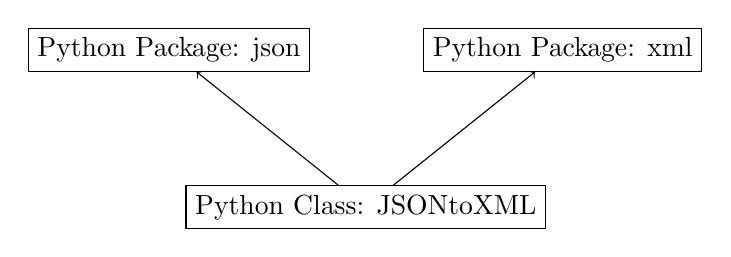
\begin{tikzpicture}
    \node[draw] (json) at (0,0) {Python Package: json};
    \node[draw] (xml) at (5,0) {Python Package: xml};
    \node[draw] (jsontoxml) at (2.5,-2) {Python Class: JSONtoXML};

    \path [->] (jsontoxml) edge node {} (json);
    \path [->] (jsontoxml) edge node {} (xml);
\end{tikzpicture}
\end{center}
\caption{An example of a module view which illustrates the dependencies of the \texttt{JSONtoXML} class}
\end{subfigure}
\caption{A simple module view of a JSON to XML program.}
\end{figure}

\section{Component-and-Connector Views}
Component-and-connector views focus on the runtime, or dynamic behaviour of a system.
Components are units which perform some computation or operation at runtime.
These components could overlap with the modules of a module view but are often at a higher level of abstraction.
The focus of component-and-connector views is how these components communicate at runtime.
Runtime communication is the connector of components.
For example, a service which registers users to a website might have new registrations communicated via a \link{REST}{https://www.ibm.com/cloud/learn/rest-apis} request.
The service may then communicate the new user information to a database via SQL queries.

When we look at software architecture, component-and-connector views are the most commonly used views.
They are common because they contain runtime information which is not easily automatically extracted.
Module views can be generated after the fact, i.e. it is easy enough for a project to generate a UML inheritance diagram.
Component-and-connector views are often something that are maintained manually by architects and developers.

\section{Allocation Views}
According to Bass et al, allocation views map the software's structures to the system's non-software structures \cite{bass2021software}.
They include concepts such as who is developing which software elements,
where are source files stored for different activities such as development and testing,
and where are software elements executed.
The first two points are important for project management and build management.
The last point of how the software is executed on different processing nodes is important for architectural design.
This is sometimes called the \emph{deployment structure} or the software system's \emph{physical architecture}.

Understanding the physical architecture (simplistically the hardware\footnote{Whether it is virtualised or physical hardware}
on which the software is executed) is important when designing the software's \emph{logical architecture}.
Component-and-connector views describe the software's logical architecture.
This design of the logical architecture must contain components that can be allocated appropriately to processing nodes,
and these nodes must have communication links that enable the components to interact.

\section{On-line Store Example}
Consider a simple on-line store selling a number of different products. Customers can use both web and mobile applications to shop at the store.
The architecture is designed to support the functional requirement that a customer can start shopping on one device and continue on another device.

\subsection{Allocation View}
Figure \ref{fig:deploymentDiagram} is an example allocation view of the system.
It is a UML deployment diagram showing the system's physical architecture
and some of the components that are deployed onto that structure.
For simplicity, details such as load balancing and failover are not shown in this example.

\begin{figure}[h]
    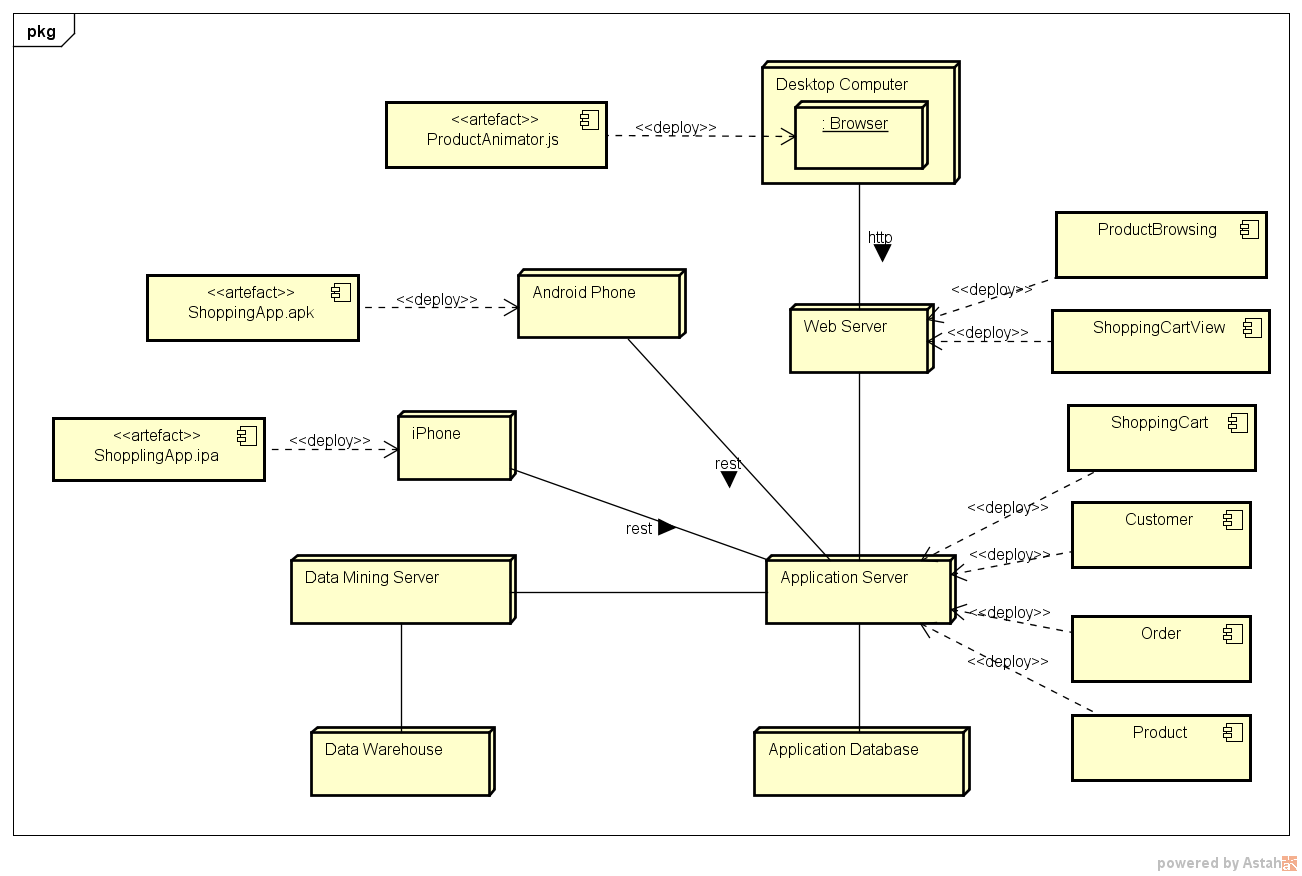
\includegraphics[trim=37 57 20 40,clip,width=\textwidth]{images/deployment_diagram.png}
    \caption{Example allocation view for an on-line store.}
    \label{fig:deploymentDiagram}
\end{figure}

\noindent
There are both web and mobile applications that allow customers to shop at the store.
A J2EE server (e.g. \link{TomEE}{https://tomee.apache.org/}), running on a web server hardware platform,
handles browser requests from customers, using the HTTP protocol over the Internet.
A JavaScript module called \texttt{ProductAnimator} is downloaded to the customer's browser to allow them to see interactive 3d views of products.
The \texttt{ProductBrowsing} and \texttt{ShoppingCartView} components run on the J2EE server, providing those aspects of the user interaction.
The J2EE server uses RMI\footnote{Remote Method Invocation} over a network connection to an application server.

The application server provides the core logic of the on-line store.
Examples of components that would run on the application server are \texttt{Customer}, \texttt{ShoppingCart}, \texttt{Order} and \texttt{Product}.
The application server uses JPA\footnote{Java Persistence API} over a network connection to a server running the application database.
The application server also uses RMI over a network connection to communicate with a data mining server.

The data mining server uses JDBC\footnote{Java DataBase Connectivity} over a network connection to a server running the data warehouse.
The mobile applications run on their respective phone environments and use REST API calls over the Internet to interact with application server.

\subsubsection{Deployment Diagram Notation}\label{sec:deploymentNotation}
In the diagram, cube icons represent \emph{nodes}. Nodes are computational resources that can execute software artifacts.
Nodes may be \guillemotleft device\guillemotright's, representing hardware.
They may also be \guillemotleft executionEnvironment\guillemotright's, representing software that provides an environment in which other software artifacts can be executed.
(The keyword has been shortened to \guillemotleft exec env\guillemotright~in this example.)
Execution environments need to be allocated to devices.
In figure \ref{fig:deploymentDiagram}, \texttt{Browser} and \texttt{J2EE Server} are software environments running,
respectively, on the hardware devices \texttt{Personal Computer} and \texttt{Web Server}.

The solid lines between nodes are \emph{associations}, which represent communication paths.
A communication path can represent a \emph{physical connection} or \emph{protocol}.
Formally, a stereotype (e.g. \guillemotleft protocol\guillemotright) is used to distinguish the type of communication path.
In figure \ref{fig:deploymentDiagram}, all communication paths are protocols so the stereotype is not included.
The protocol name is used to indicate which one is being used on the communication path.
The end of an association can indicate \emph{multiplicity}.
In a deployment diagram this is used to indicate that some nodes may be replicated
(e.g. for performance or robustness). The `*' symbol is used to indicate many instances may be involved.

The rectangles with a `plug' icon in their top-right corner are \emph{components}.
Components are executable software which need to be deployed to a node on which they will run.
The dashed dependency arrow, with the stereotype \guillemotleft deploy\guillemotright, indicates the node on which the component will be deployed for execution.

\textbf{Note}, this approach of showing components being deployed to nodes is an older style of UML.
The current version of UML has the concept of \emph{artifacts} being deployed to nodes.
Artifacts can implement (manifest in UML terminology) components, which provides an additional layer of abstraction.
Formally, components would be manifested by an artifact that is then deployed to a node.
In figure \ref{fig:deploymentDiagram}, components are deployed directly to nodes to keep the diagram simple.
UML provides multiple ways to indicate which artifacts are deployed on a node, e.g. a textual list of artifacts inside the node icon.
The approach taken for a diagram should be chosen to aid readability and reduce clutter.

Artifacts are used in this diagram to represent software that has to be packaged
(i.e. deployed through a manifest), which corresponds to the idea of an artifact in the note above.
An artifact is represented by a rectangle with the \guillemotleft artifact\guillemotright~keyword and the name of the artifact that is created for deployment.

\subsection{Component-and-Connector View}
Figure \ref{fig:componentDiagram} is an example component-and-connector view of a small part of the system.
It is a UML component diagram showing the logical architecture of the components that allow customers to browse for products and add them to their shopping cart.

\begin{figure}[h]
    \centering
    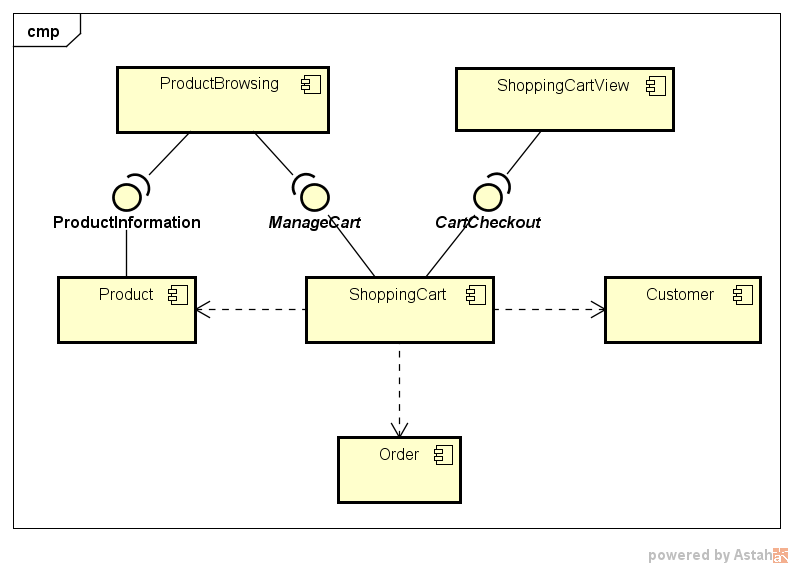
\includegraphics[trim=37 48 18 50,clip,width=0.75\textwidth]{images/component_diagram.png}
    \caption{Example component-and-connector view for part of an on-line store.}
    \label{fig:componentDiagram}
\end{figure}

\noindent
As was shown in figure \ref{fig:deploymentDiagram}, the \texttt{ProductBrowsing} and \texttt{ShoppingCartView} components are deployed on the J2EE server.
These two component provide the user interaction behaviour of browsing for products, adding them to the shopping cart, and purchasing the products.

The \texttt{Product}, \texttt{ShoppingCart}, \texttt{Order} and \texttt{Customer} components are deployed on the application server.
These components deliver the logical behaviour of providing information about products, tracking what is in the shopping cart, and placing orders.

The \texttt{ProductBrowsing} component uses the \texttt{\textsl{ProductInformation}} and \texttt{\textsl{ManageCart}} interfaces.
These two interfaces are realised (or implemented) by the \texttt{Product} and \texttt{ShoppingCart} components respectively.
The \texttt{ShoppingCartView} component uses the \texttt{\textsl{CartCheckout}} interface, which is realised by the \texttt{ShoppingCart} component.
These interfaces describe the communication pathways between the components on the different nodes of the physical architecture.

The \texttt{ShoppingCart} component uses the \texttt{Product}, \texttt{Customer} and \texttt{Order} components.
At the programming level, there could be interfaces between these components which are not shown in this diagram.

\subsubsection{Component Diagram Notation}\label{sec:componentNotation}
As indicated in \ref{sec:deploymentNotation}, rectangles with the `plug' icon represent \emph{components} in UML.

Circles represent \emph{interfaces}, and are labelled with the interface's name.
A line from a component to an interface circle indicates that the component provides (or realises) the interface.

Cups represent a \emph{required interface}, and a line from a component to a cup indicates that the component depends on (or uses) the interface.
This notation visualises the connection between components.

Dependency arrows point from a component whose runtime behaviour depends on behaviour provided by the target component.

\subsection{Module View}
Figure \ref{fig:classDiagram} is an example module view that is a UML class diagram showing the static structure of the classes that implement the \texttt{ShoppingCart} component.
To keep the diagram simple, most operations and attributes are not shown and only the classes and interfaces related to adding items to a shopping cart and checking out are shown.

\begin{figure}[h]
    \centering
    \begin{adjustwidth}{-9mm}{-10mm}
        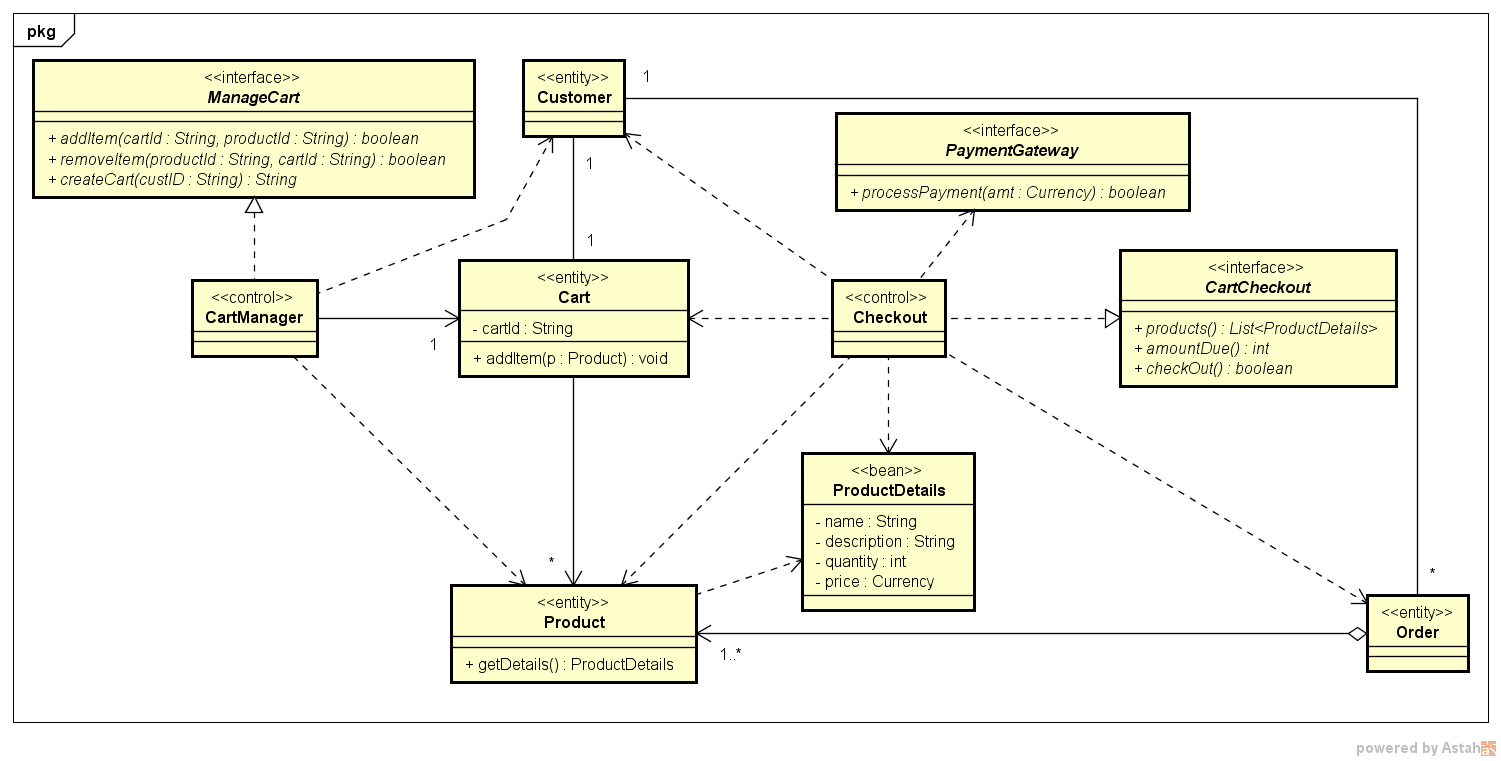
\includegraphics[trim=24 51 23 43,clip,width=0.97\paperwidth]{images/shopping_cart_class_diagram.png}
    \end{adjustwidth}
    \caption{Example module view for part of the shopping cart package in the class model.}
    \label{fig:classDiagram}
\end{figure}

\noindent
The \texttt{CartManager} and \texttt{Checkout} control classes implement, respectively, the \texttt{\textsl{ManageCart}} and \texttt{\textsl{Cart\-Checkout}} interfaces.
These two classes implement the Façade design pattern and manage how adding items to a shopping cart and checking out are delivered by the classes in this package.
Going back to the component and connector view (figure \ref{fig:componentDiagram}),
when a customer, via their web browser, selects to add a product to their shopping cart,
the \texttt{ProductBrowsing} component's logic uses the \texttt{\textsl{ManageCart}} interface's \texttt{additem} operation to send a message to the \texttt{ShoppingCart} component.
The \texttt{CartManager} class would load the product details from the application database, using the \texttt{productId} (details not shown in this diagram),
create a \texttt{Product} object to represent it, and add that object to the \texttt{Cart} specified by the \texttt{cartId}.

When a customer wants to checkout the products in their shopping cart, the \texttt{ShoppingCartView} component
uses the \texttt{\textsl{Checkout}} interface's \texttt{products} operation to get a list of the product details to be displayed in the shopping cart.
The \texttt{ProductDetails} class is a Java bean that is used to pass the data about each product to the \texttt{ShoppingCartView}.
Once a customer decides to buy the products in their shopping cart, the \texttt{ShoppingCartView} sends the \texttt{checkOut} message to the \texttt{ShoppingCart}.
\texttt{Checkout} uses the \texttt{\textsl{PaymentGateway}} interface to process the payment.

\subsubsection{Class Diagram Notation}\label{sec:classNotation}
Formally in UML, rectangles represent \emph{classifiers}. A \emph{class} is one type of classifier.
In a class diagram, a rectangle represents a class, unless a keyword is used to indicate that it is a different type of classifier.
Classifier rectangles have three compartments.
The top compartment contains its name and optionally includes a keyword, stereotypes and properties for the classifier.
The middle compartment contains \emph{attributes}.
The bottom compartment contains \emph{operations}.

Solid lines represent \emph{associations}, which may optionally have an arrow indicating the direction of the relationship.
An association indicates a structural relationship between classes.
Typically this means that the target of an association will be an implicit attribute of the class.
The end of an association can use \emph{multiplicity} to indicate the number of objects of the class that may take part in the relationship.
A diamond on the end of an association indicates \emph{aggregate} relationship.
The diamond is on the end that is the aggregate, and the other end is the part.
The diamond may be filled or not. A filled diamond represents \emph{composition} in UML.
This indicates `ownership', where the aggregate controls the lifespan of the part.
A hollow diamond, as in the relationship between \texttt{Order} and \texttt{Product},
indicates \emph{aggregation} in UML.
This is a weaker relationship than composition, as the aggregate does not control the lifespan of the part,
but it still indicates a strong relationship between the classes.

A dashed line with an open arrowhead (e.g. from \texttt{CartManager} to \texttt{Product})
indicates that one classifier \emph{depends} on (or uses) another. This is meant to indicate a transient relationship.

A dashed lines with a closed and hollow arrowhead (e.g. from \texttt{Checkout} to \texttt{\textsl{CartCheckout}})
indicates that the class is \emph{realising} (or implementing) that interface.

\textit{Italicised} names indicate an abstract classifier. Keywords are used to indicate the type of a classifier.
In this example, the keyword \guillemotleft interface\guillemotright~indicates that the classifier is an interface.
Stereotypes use the same notation as keywords. Three standard stereotypes for classes in UML are:
\begin{description}[nosep,left=5mm]
    \item[\guillemotleft entity\guillemotright] An entity (or concept) from the problem domain.
    \item[\guillemotleft control\guillemotright] Provides logical behaviour from the solution domain.
    \item[\guillemotleft boundary\guillemotright] Communicates with something outside of the system. (Not shown in diagram.)
\end{description}
An additional stereotype \guillemotleft bean\guillemotright~is used to indicate that the class is a Java bean.

\section{C4 Model}
Simon Brown's C4 model provides a set of abstractions that describe the static structure of the software architecture \cite{brown2022c4}.
The C4 model provides a hierarchical set of views leading to finer levels of detail.
The hierarchical structure is based on the idea that a software system is composed of containers, which are implemented by components, that are built using code.
\begin{description}
    \item[Software System] Represents something that delivers value to it users (human or other system).
    \item[Containers] Deployable `block' of code or data that provides behaviour in the software system.
    \item[Components] Encapsulate a group of related functionality, which is hidden behind a published interface.
    \item[Code] Elements built from programming language constructs, e.g. classes, interfaces, functions, ....
\end{description}

\begin{figure}[h]
    \centering
    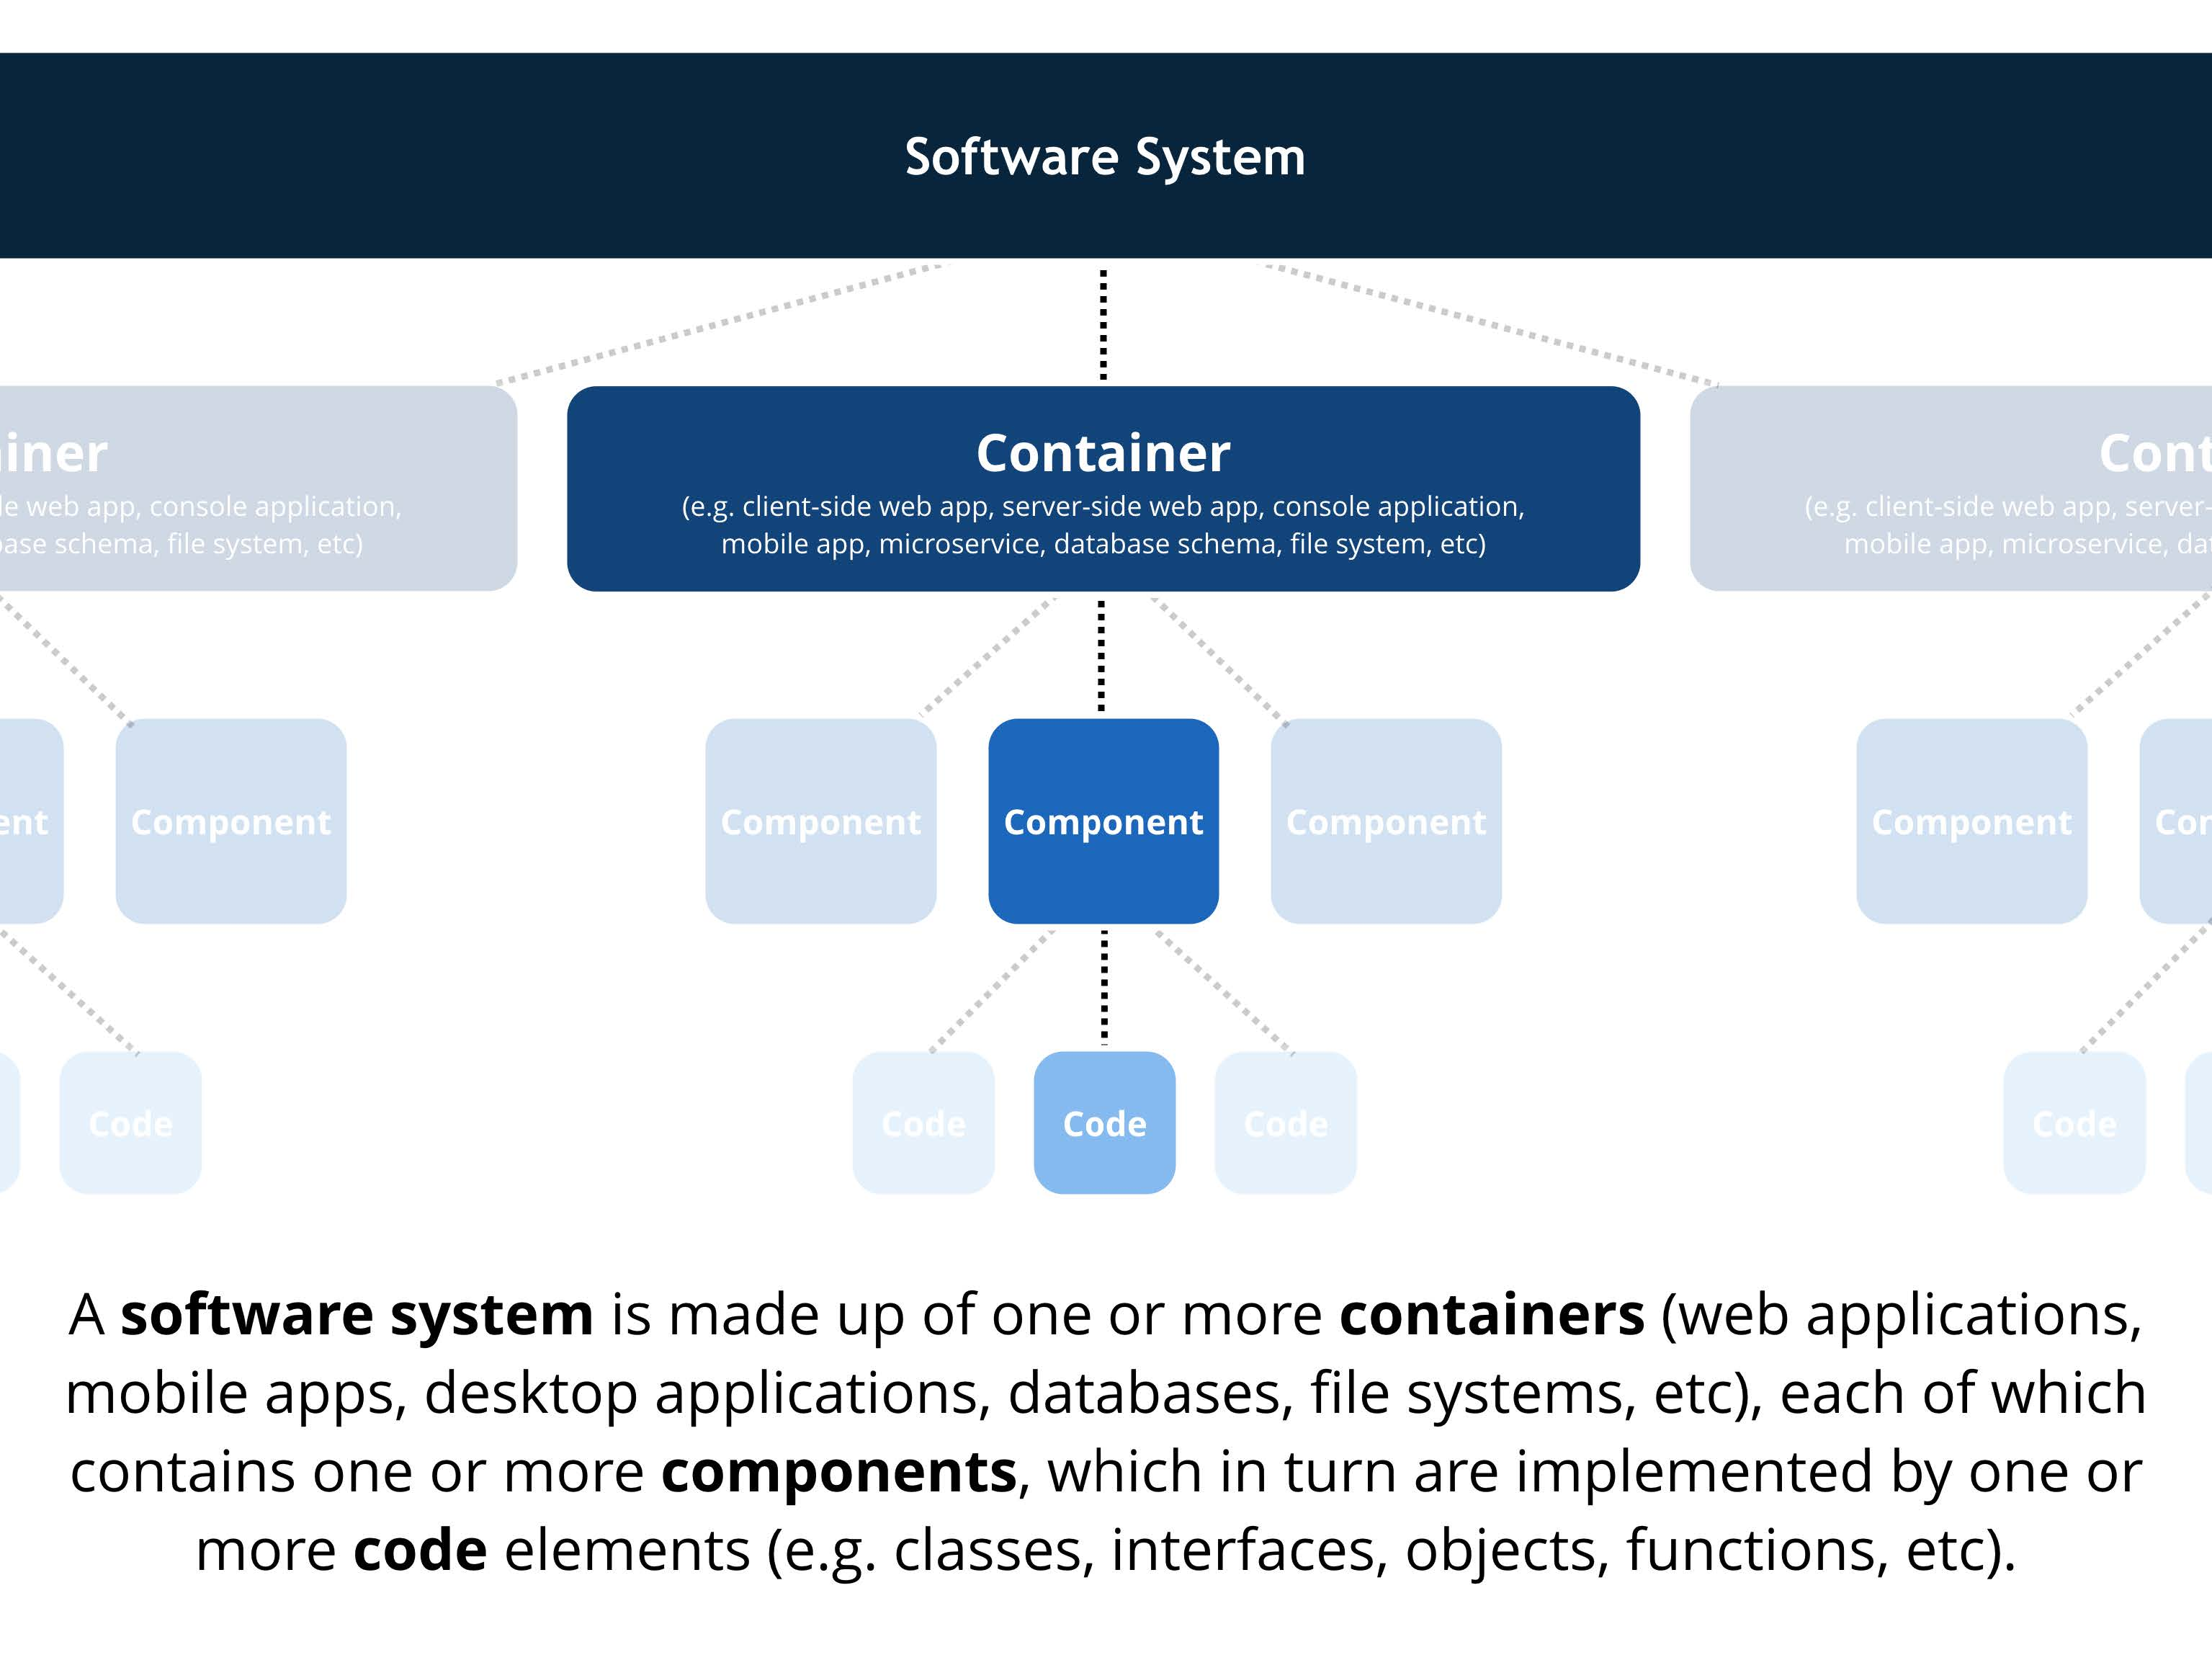
\includegraphics[trim=0 8 0 5,clip,width=0.8\textwidth]{images/c4_terminology.jpg}
    \caption{Levels within the C4 model (figure 2.1 from \cite{brown2022c4}).}
    \label{fig:c4terms}
\end{figure}

\noindent
This leads to describing the static structure of software architecture through four levels of abstraction.
Each level provides detail about each part of the previous level.
\begin{description}
    \item[Context] How the software system fits into the broader context around it.
    \item[Containers] How the containers are connected to deliver system functionality.
    \item[Components] How the components are structured to implement a container's behaviour.
    \item[Code] How the code is structured to implement a component.
\end{description}

\noindent
The software system's context and container views provide an overview of the software architecture.
The context describes the software system's scope, users and external dependencies.
Containers describe the main structure of the software system and the technologies selected.
Examples of containers would be web or mobile applications, databases, message buses, ....
Decisions about how to structure containers will have major implications for how the components and code will be designed.

The component view describes the major parts of a container and how they are connected.
This includes the important responsibilities of each component, their public interfaces, and technology choices.
Examples of technology choices at the component level would be using Node.js and React to implement a web application, 
and React Native to implement the mobile apps.



\section{4+1 Views}
These notes have adopted the approach advocated by Bass et al \cite{bass2021software}.
Other experts in the field have advocated other views to describe software architecture.
Phillipe Krutchen was one of the earliest to advocate the idea of using views to document software architectures.
In the article ``4+1 View Model of Software Architecture'' \cite{4+1-model} he describes five different views.
These are logical, process, development, physical and scenario views, which are described below.
\begin{description}
    \item[Logical] How functionality is implemented, using class and state diagrams.
    \item[Process] Runtime behaviour, including concurrency, distribution, performance and scalability.
                            Sequence, communication and activity diagrams are used to describe this view.
    \item[Development] The software structure from a developer's perspective, using package and component diagrams.
                                    This is also known as the implementation view.
    \item[Physical] The hardware environment and deployment of software components.
                            This is also known as the deployment view.
    \item[Scenario] Interactions between objects and between processes to deliver functional requirements.
                             This is the `+1' view as it is used to validate the software architecture.
                             This is also known as the use case view.
\end{description}

\section{Conclusion}
Architectural views help developers understand the different dimensions and details of a complex software architecture.
As a software architect you need to choose which views provide meaningful information about your software system.
The graphical notation used to describe a view is only one part of the view (though an important part).
